\section{Finite Fields and Bit Lengths}
\label{sec:finiteFieldsAndBitLengths}

\noindent
For those who go through the Nightfall code, you mght realise there are many number conversions being made in the zkp microservice. In particular, there are frequently conversions and restrictions to $216$-bit ($27$-byte) values in much of today's Nightfall code. These conversions are a consequence of working with zk-SNARKs.\\
\\
Like many cryptographic protocols, zk-SNARKs make use of representing numbers as points on an elliptic curve. In doing so, the results of our computations become quite difficult to `unravel' -- that is, given an output, it becomes computationally infeasible for someone to determine the inputs. However, it also restricts the mathematics we can do. This is a gross oversimplification of why elliptic curves are used, but let's talk about them.\\
\\
Currently on Ethereum, there is only one elliptic curve for which it is `cheap' (in terms of gas costs) to perform calculations (due to there being precompile contracts supporting calculations on this curve):
\begin{align*}
    E := y^2 = x^3 + 3
\end{align*}

This curve looks like this:
\begin{figure}[H]
	\begin{center}
		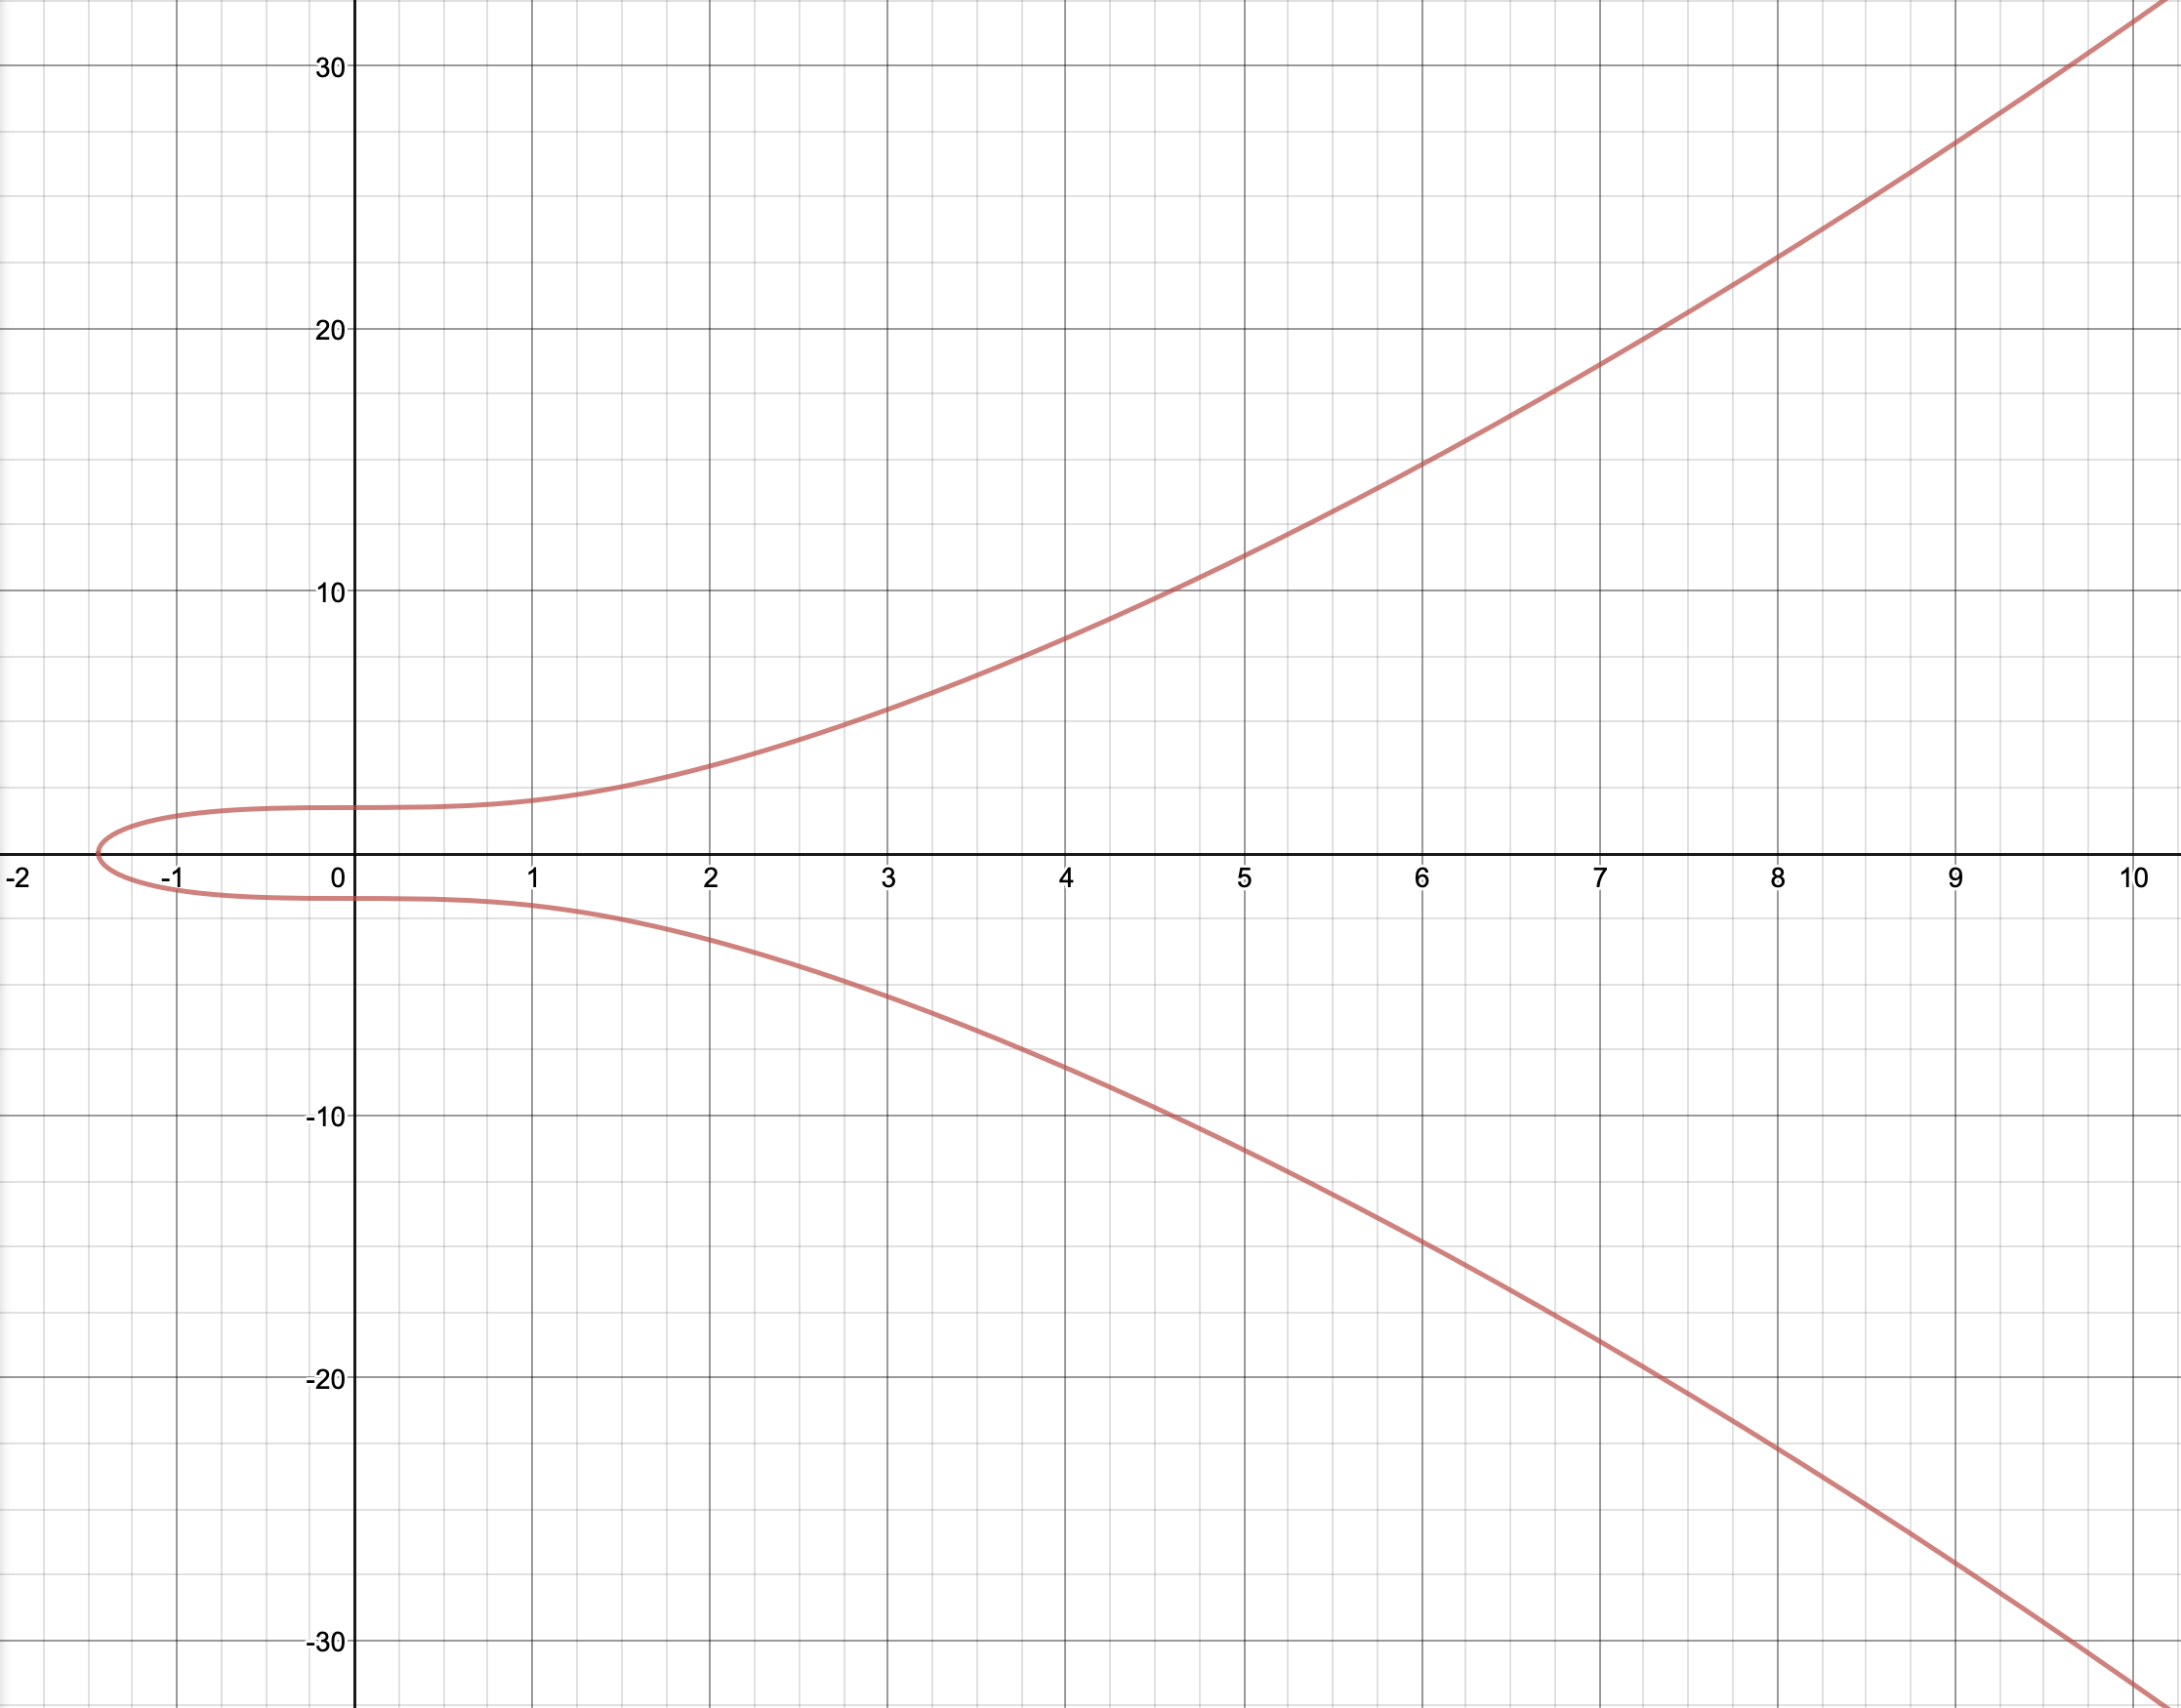
\includegraphics[width=0.8\textwidth]{images/ellipticCurveReals.png}
	\end{center}
	\caption{$y^2 = x^3 + 3$ over the real numbers.}
	\label{pic:ftShield}
\end{figure}

As an example, let's restrict the $x$ and $y$ coordinates to be the field of integers modulo $7$. I.e. we only allow the numbers $\mathbb{F}_7 = {0, 1, 2, 3, 4, 5, 6}$. In this world, $5 + 5 = 10 = 3\;(mod\;7)$.\\
\\
Let's consider the possible $y$-values of our elliptic curve $E$ when restricted to $\mathbb{F}_7$ (note: we write $E[\mathbb{F}_7]$ for 'the elliptic curve defined over the finite field $\mathbb{F}_7$).

\begin{tabular}{|c|c|c|c|c|c|c|c|}
    \hline
    $y$ & $0$ & $1$ & $2$ & $3$ & $4$ & $5$ & $6$ \\
    \hline
    $y^2$ & $0$ & $1$ & $4$ & $9=2$ & $16=2$ & $25=4$ & $36=1$ \\
    \hline
\end{tabular}

Now let's consider the $x$-values of $E[\mathbb{F}_7]$:

\begin{tabular}{|c|c|c|c|c|c|c|c|}
    \hline
    $x$ & $0$ & $1$ & $2$ & $3$ & $4$ & $5$ & $6$ \\
    \hline
    $x^3$ & $0$ & $1$ & $8=1$ & $27=6$ & $64=1$ & $125=6$ & $216=6$ \\
    \hline
    $x^3+3$ & $3$ & $4$ & $4$ & $9=2$ & $4$ & $9=2$ & $9=2$ \\
    \hline
    $= y^2$ & - & $4$ & $4$ & $2$ & $4$ & $2$ & $2$ \\
    \hline
    Valid $y$-values & 
        -- & 
        \makecell{$2$\\$5$} &
        \makecell{$2$\\$5$} &
        \makecell{$3$\\$4$} &
        \makecell{$2$\\$5$} &
        \makecell{$3$\\$4$} & 
        \makecell{$3$\\$4$} \\
    \hline
\end{tabular}

So we have a set of valid points of $\infty, (1,2), (1,5), (2,2), (2,5), (3,3), (3,4), (4,2), (4,5), (5,3), (5,4), (6,3), (6,4)$.\\
\\
These $13$ points are the only points which exist on $E[\mathbb{F}_7]$. $E[\mathbb{F}_7]$ is a `group' of order $13$.\\
In other words: the curve $E: y^2 = x^3 + 3$ --- when restricted to the $7$ values of $\mathbb{F}_7$ --- produces a group $E[\mathbb{F}_7]$ of order $13$.\\
\\
We superimpose the points of $E[\mathbb{F}_7]$ (in green) below:
\begin{figure}[H]
	\begin{center}
		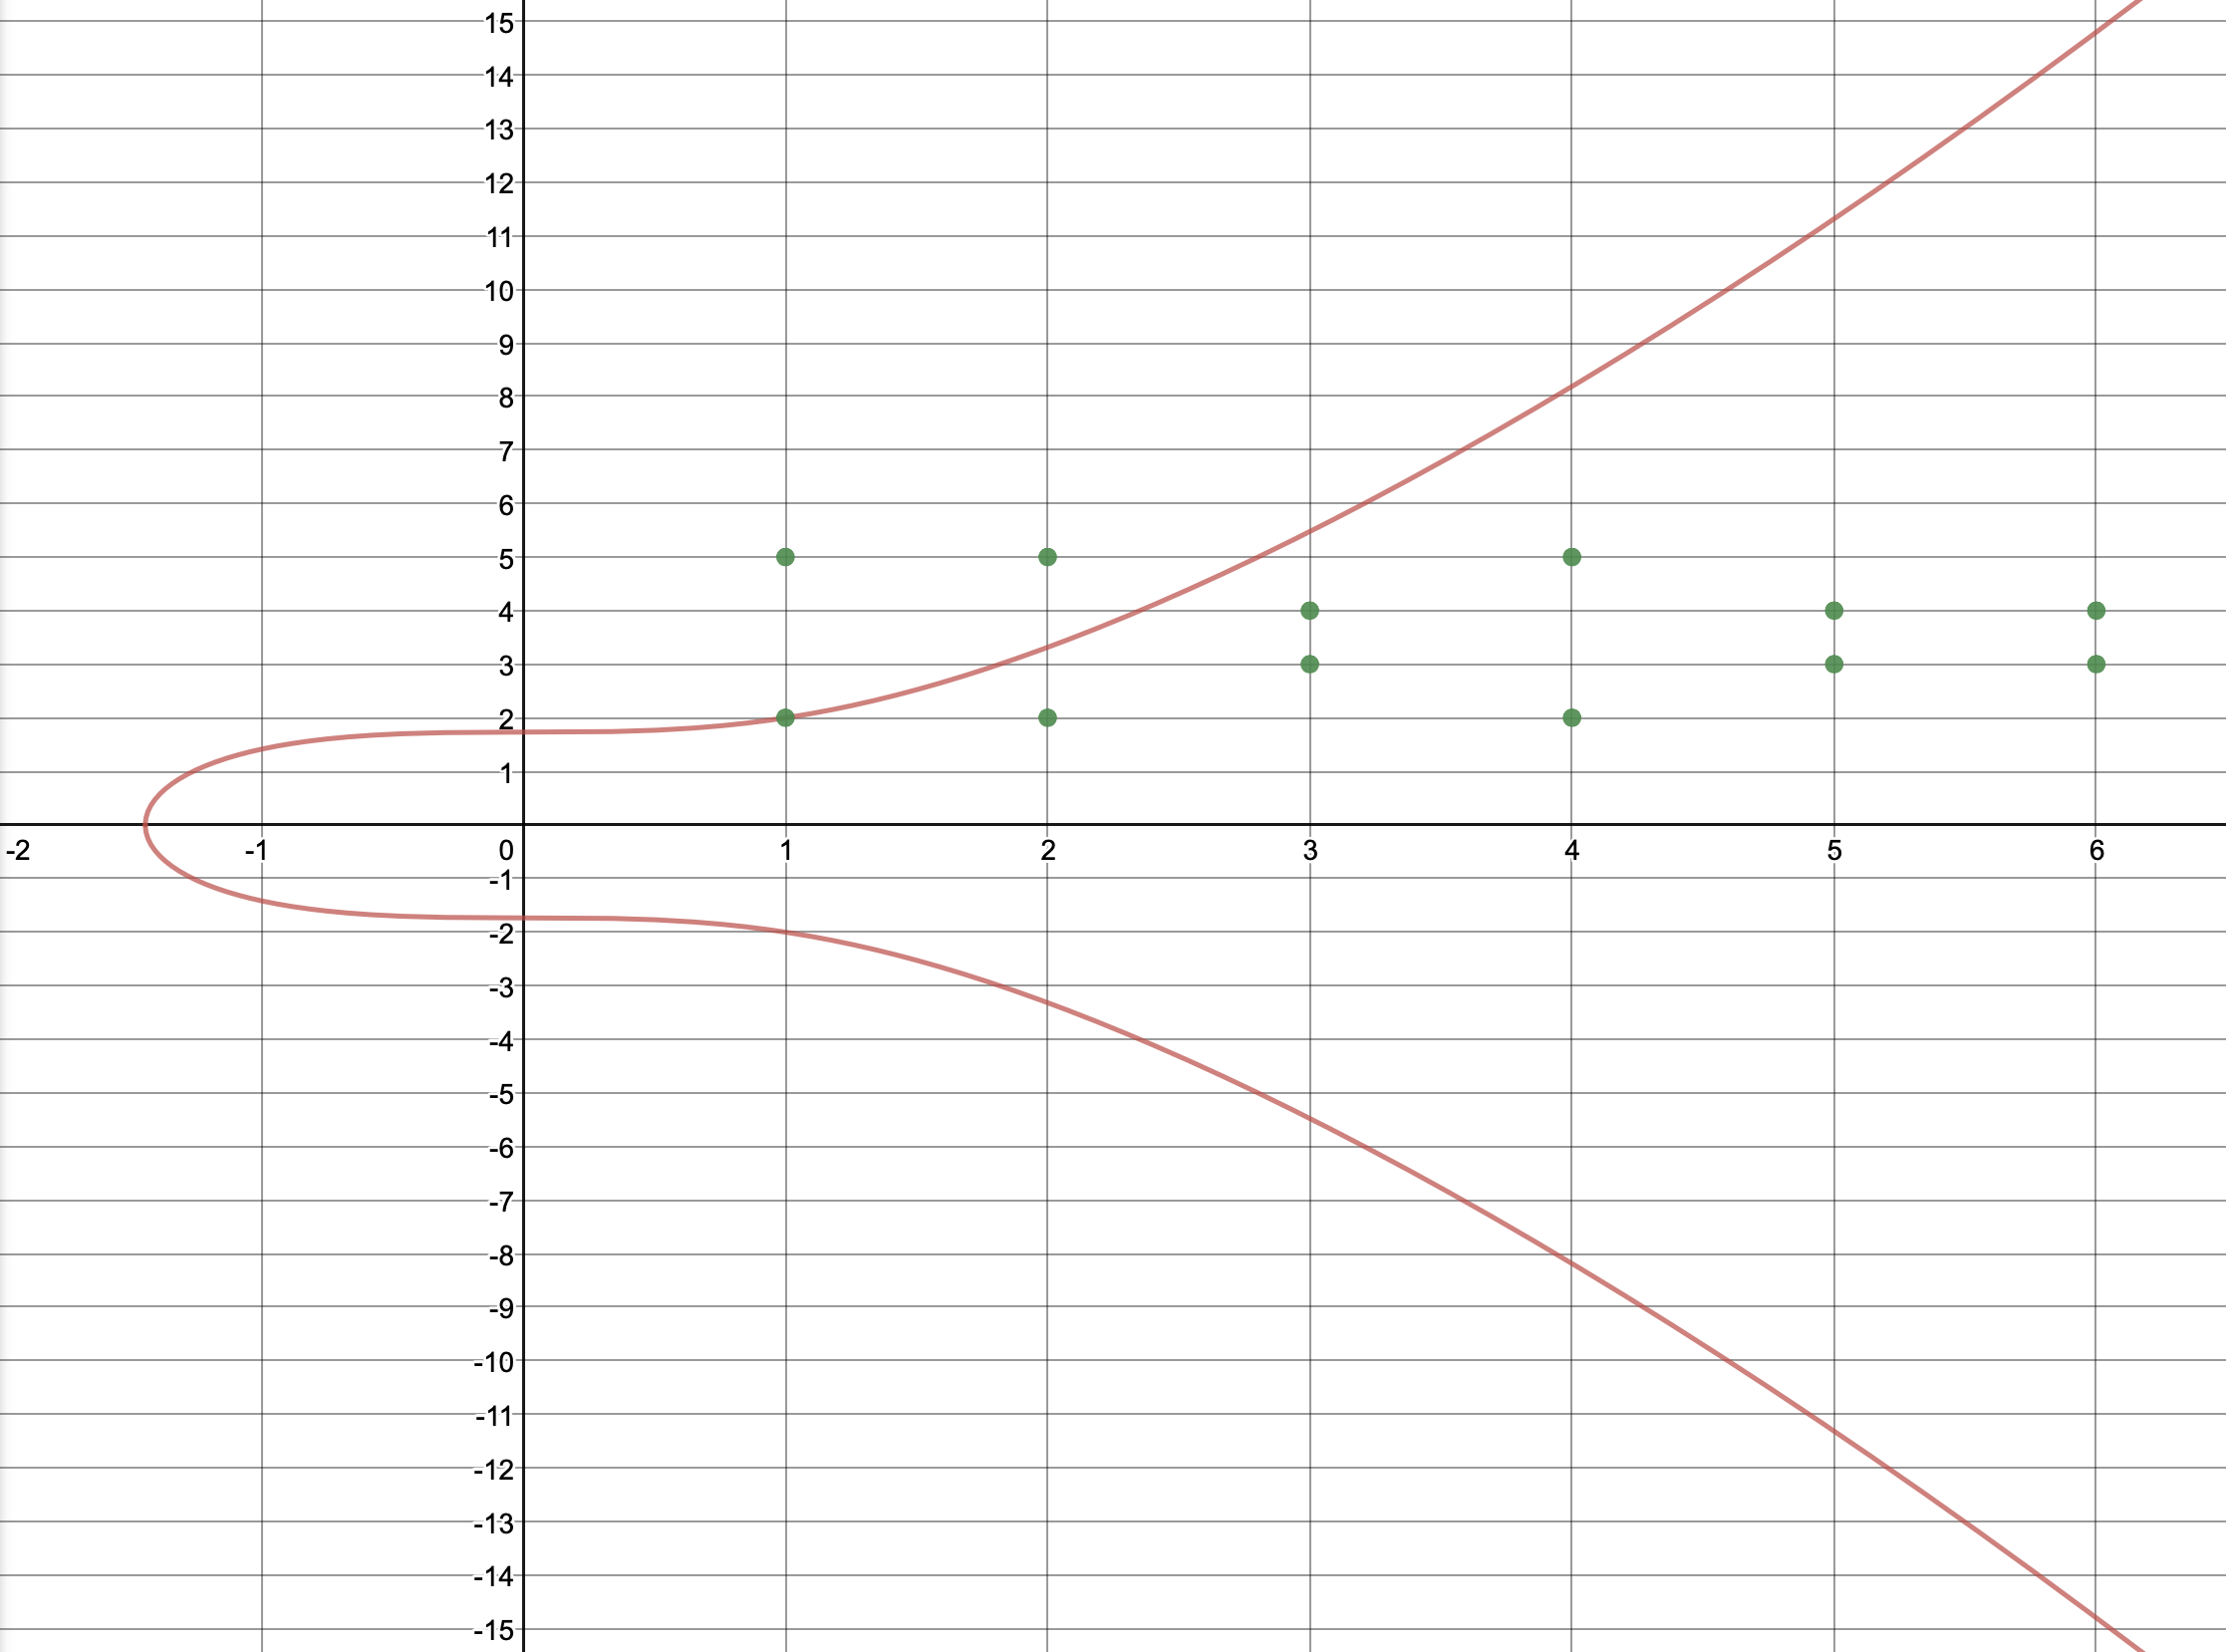
\includegraphics[width=0.8\textwidth]{images/ellipticCurveF7.png}
	\end{center}
	\caption{$y^2 = x^3 + 3$ over $\mathbb{F}_7$ shown as green dots.}
	\label{pic:ftShield}
\end{figure}

An important thing to take away from this example, is that there are 3 distinct things for us to be aware of: an elliptic curve equation $E$, a finite field $\mathbb{F}$, and the resulting group $G = E[\mathbb{F}]$. Sometimes the number of elements in the group $G$ is \textit{more than} the number of elements in the field $\mathbb{F}$ (as in the above example), and sometimes the number of elements in the group $G$ is \textit{less than} the number of elements in the field $\mathbb{F}$ (as we will see is the case with Ethereum).\\
\\
In practice, the finite field $\mathbb{F}_p$ used in Ethereum is of size
\begin{align*}
    p = 21888242871839275222246405745257275088696311157297823662689037894645226208583
\end{align*}

The elliptic curve $E: y^2 = x^3 + 3$, when restricted to the $p$ values of $\mathbb{F}_p$, produces a group $G_1 = E[\mathbb{F}_p]$ of prime order
\begin{align*}
    q = 21888242871839275222246405745257275088548364400416034343698204186575808495617
\end{align*}

I.e. $G_1 = E[\mathbb{F}_p]$ is a group with $q$ distinct points. Here, $q < p$; the size of the group $G_1$ is less than the size of the field $\mathbb{F_p}$.\\
\\
This has an important consequence when working within ZoKrates. To generate zk-SNARKs, ZoKrates will convert the numbers we pass as inputs to our off-chain calculation (as well as all intermediate numbers of the calculation) into elliptic curve points. To tie-in with Ethereum, ZoKrates converts all of the numbers used in its calculations into elements of the group $G_1$. Therefore, we need to make sure that \textbf{all} of the inputs we pass into ZoKrates are \textbf{less than} the size of the group $G_1$, $q = 21888242871839275222246405745257275088548364400416034343698204186575808495617$.\\
\\
This value of $q$ is slightly less than $254$-bits. I.e. $2^{253} < q < 2^{254}$.\\
\\
Hence, to be sure we don't `overflow' modulo-$q$, it's safest to only pass numbers to ZoKrates which are $\leq 253$-bits. When working with Ethereum, we often work with hex numbers (because Solidity `likes' hex numbers), which means it's often nice for the bit-length we work with to be divisible by $8$. Since $248$ is the largest number below $253$ which is divisible by $8$, this would have been a nice choice for all of the numbers Nightfall passes to ZoKrates.\\
\\
However, you might notice we instead restrict all our numbers to $216$-bits. The reason for this is the maximum size of a message in the NIST specification of the sha256 hashing algorithm. The largest message size for `one round' of sha256 hashing is $447$-bits. The version of ZoKrates used in Nightfall currently only supports `one round' of sha256 hashing. Hence our inputs to each hashing iteration must be $447$-bits or less.\\
\\
You'll see in the protocols below, that we frequently need to concatenate two values and then hash them. Hence we need each of the two values to be at most $223$-bits to fit inside `one round' of sha256 hashing. Given that we also prefer bit-lengths which are divisible by $8$, $216$-bits becomes the best choice for our purposes.\\
\\
\textbf{And that's why you'll see conversions and restrictions to 216-bit (27-byte) values in much of today's Nightfall code.}\\
\\
In cases where we need to use a number with a greater bit-length than $216$ (for security purposes), we deconstruct that number into an array of $216$-bit values. E.g. a $512$-bit number might be deconstructed into an array [$80$-bits, $216$-bits, $216$-bits].
